\documentclass{standalone}
\usepackage{tikz}
\usetikzlibrary{patterns, positioning}

\begin{document}
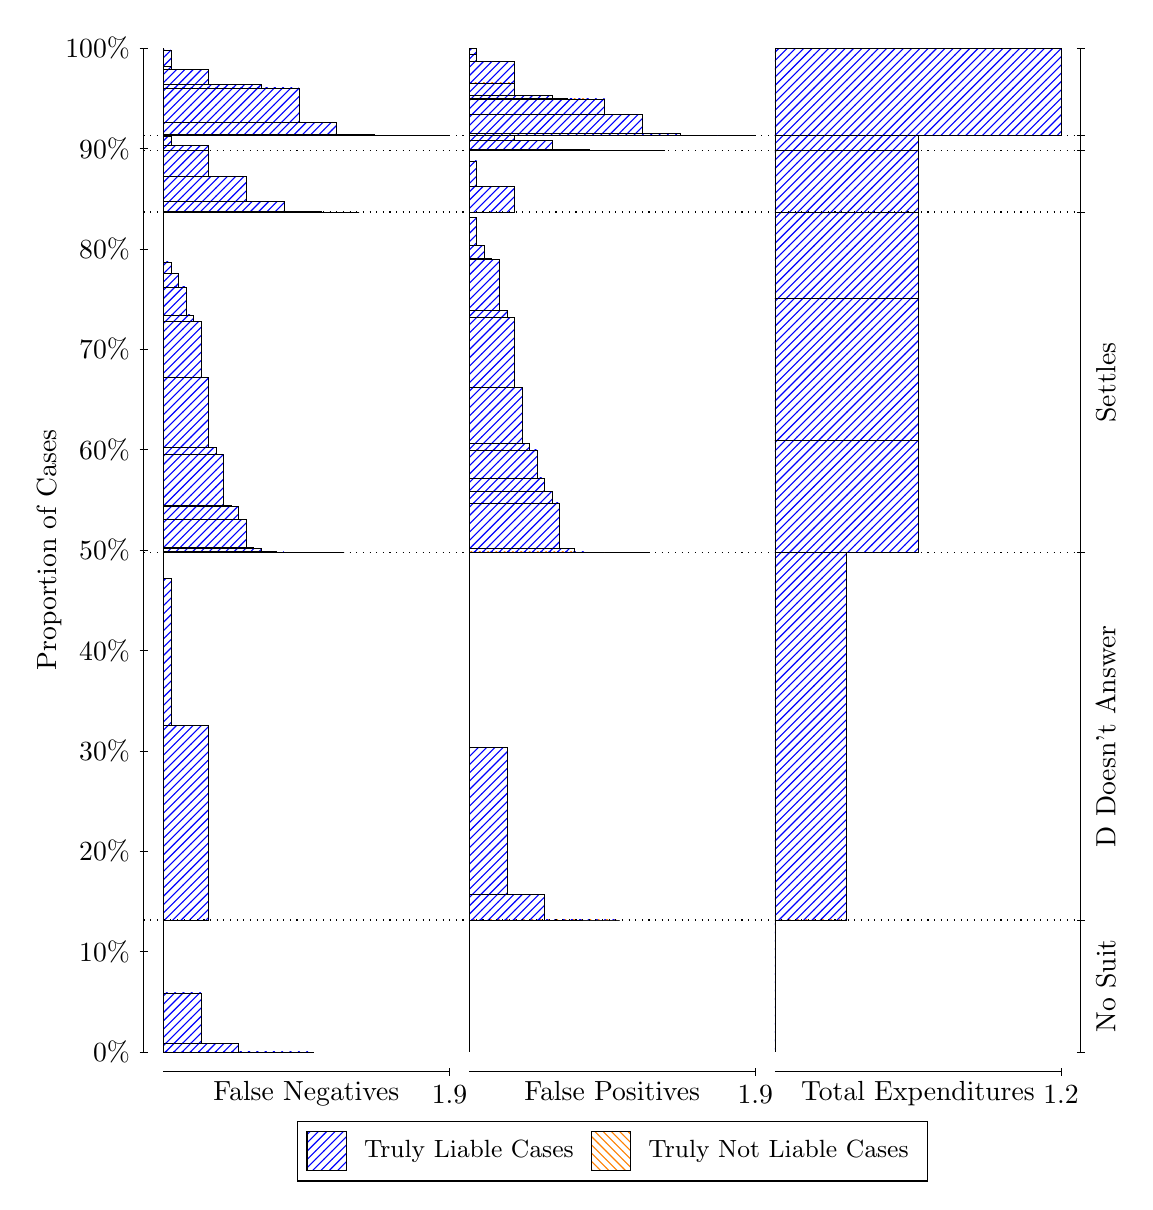
\begin{tikzpicture}
\draw[black, very thin] (1.5,1.75) -- (1.5,14.5);
\node[rotate=90, anchor=center] at (0.3, 8.125) {Proportion of Cases};
\draw[black, very thin] (1.45,1.75) -- (1.55,1.75);
\node[anchor=east] at (1.45, 1.75) {0\%};
\draw[black, very thin] (1.45,3.025) -- (1.55,3.025);
\node[anchor=east] at (1.45, 3.025) {10\%};
\draw[black, very thin] (1.45,4.3) -- (1.55,4.3);
\node[anchor=east] at (1.45, 4.3) {20\%};
\draw[black, very thin] (1.45,5.575) -- (1.55,5.575);
\node[anchor=east] at (1.45, 5.575) {30\%};
\draw[black, very thin] (1.45,6.85) -- (1.55,6.85);
\node[anchor=east] at (1.45, 6.85) {40\%};
\draw[black, very thin] (1.45,8.125) -- (1.55,8.125);
\node[anchor=east] at (1.45, 8.125) {50\%};
\draw[black, very thin] (1.45,9.4) -- (1.55,9.4);
\node[anchor=east] at (1.45, 9.4) {60\%};
\draw[black, very thin] (1.45,10.675) -- (1.55,10.675);
\node[anchor=east] at (1.45, 10.675) {70\%};
\draw[black, very thin] (1.45,11.95) -- (1.55,11.95);
\node[anchor=east] at (1.45, 11.95) {80\%};
\draw[black, very thin] (1.45,13.225) -- (1.55,13.225);
\node[anchor=east] at (1.45, 13.225) {90\%};
\draw[black, very thin] (1.45,14.5) -- (1.55,14.5);
\node[anchor=east] at (1.45, 14.5) {100\%};

\draw[black, very thin] (13.4,1.75) -- (13.4,14.5);
\draw[black, very thin] (13.35,1.75) -- (13.45,1.75);
\node[anchor=west] at (13.35, 1.75) {};
\draw[black, very thin] (13.35,3.4262) -- (13.45,3.4262);
\node[anchor=west] at (13.35, 3.4262) {};
\draw[black, very thin] (13.35,8.0907) -- (13.45,8.0907);
\node[anchor=west] at (13.35, 8.0907) {};
\draw[black, very thin] (13.35,12.417) -- (13.45,12.417);
\node[anchor=west] at (13.35, 12.417) {};
\draw[black, very thin] (13.35,13.197) -- (13.45,13.197);
\node[anchor=west] at (13.35, 13.197) {};
\draw[black, very thin] (13.35,13.39) -- (13.45,13.39);
\node[anchor=west] at (13.35, 13.39) {};
\draw[black, very thin] (13.35,14.5) -- (13.45,14.5);
\node[anchor=west] at (13.35, 14.5) {};

\draw[black, very thin, pattern color=blue, pattern=north east lines] (1.75,1.75) rectangle (3.6623,1.75);
\draw[black, very thin, pattern color=blue, pattern=north east lines] (1.75,1.75) rectangle (3.1842,1.751);
\draw[black, very thin, pattern color=blue, pattern=north east lines] (1.75,1.751) rectangle (2.7061,1.8633);
\draw[black, very thin, pattern color=blue, pattern=north east lines] (1.75,1.8633) rectangle (2.2281,2.4999);
\draw[black, very thin, pattern color=orange, pattern=north west lines] (1.75,2.4999) rectangle (1.75,2.4999);
\draw[black, very thin, pattern color=blue, pattern=north east lines] (1.75,2.4999) rectangle (1.75,3.4262);
\draw[black, very thin, pattern color=blue, pattern=north east lines] (1.75,3.4262) rectangle (2.3237,5.8961);
\draw[black, very thin, pattern color=blue, pattern=north east lines] (1.75,5.8961) rectangle (1.8456,7.7628);
\draw[black, very thin, pattern color=orange, pattern=north west lines] (1.75,7.7628) rectangle (1.75,7.7628);
\draw[black, very thin, pattern color=blue, pattern=north east lines] (1.75,7.7628) rectangle (1.75,8.0907);
\draw[black, very thin, pattern color=blue, pattern=north east lines] (1.75,8.0907) rectangle (4.0447,8.0907);
\draw[black, very thin, pattern color=blue, pattern=north east lines] (1.75,8.0907) rectangle (3.8535,8.0907);
\draw[black, very thin, pattern color=blue, pattern=north east lines] (1.75,8.0907) rectangle (3.6623,8.0907);
\draw[black, very thin, pattern color=blue, pattern=north east lines] (1.75,8.0907) rectangle (3.5667,8.0907);
\draw[black, very thin, pattern color=blue, pattern=north east lines] (1.75,8.0907) rectangle (3.4711,8.0907);
\draw[black, very thin, pattern color=blue, pattern=north east lines] (1.75,8.0907) rectangle (3.4711,8.0907);
\draw[black, very thin, pattern color=blue, pattern=north east lines] (1.75,8.0907) rectangle (3.3754,8.0908);
\draw[black, very thin, pattern color=blue, pattern=north east lines] (1.75,8.0908) rectangle (3.2798,8.1008);
\draw[black, very thin, pattern color=blue, pattern=north east lines] (1.75,8.1008) rectangle (3.1842,8.1045);
\draw[black, very thin, pattern color=blue, pattern=north east lines] (1.75,8.1045) rectangle (3.0886,8.1046);
\draw[black, very thin, pattern color=blue, pattern=north east lines] (1.75,8.1046) rectangle (2.993,8.1046);
\draw[black, very thin, pattern color=blue, pattern=north east lines] (1.75,8.1046) rectangle (2.993,8.1473);
\draw[black, very thin, pattern color=blue, pattern=north east lines] (1.75,8.1473) rectangle (2.8974,8.1473);
\draw[black, very thin, pattern color=blue, pattern=north east lines] (1.75,8.1473) rectangle (2.8974,8.1565);
\draw[black, very thin, pattern color=blue, pattern=north east lines] (1.75,8.1565) rectangle (2.8018,8.5185);
\draw[black, very thin, pattern color=blue, pattern=north east lines] (1.75,8.5185) rectangle (2.7061,8.6818);
\draw[black, very thin, pattern color=blue, pattern=north east lines] (1.75,8.6818) rectangle (2.6105,8.682);
\draw[black, very thin, pattern color=blue, pattern=north east lines] (1.75,8.682) rectangle (2.6105,8.691);
\draw[black, very thin, pattern color=blue, pattern=north east lines] (1.75,8.691) rectangle (2.5149,8.691);
\draw[black, very thin, pattern color=blue, pattern=north east lines] (1.75,8.691) rectangle (2.5149,9.3381);
\draw[black, very thin, pattern color=blue, pattern=north east lines] (1.75,9.3381) rectangle (2.5149,9.3381);
\draw[black, very thin, pattern color=blue, pattern=north east lines] (1.75,9.3381) rectangle (2.4193,9.3383);
\draw[black, very thin, pattern color=blue, pattern=north east lines] (1.75,9.3383) rectangle (2.4193,9.4268);
\draw[black, very thin, pattern color=blue, pattern=north east lines] (1.75,9.4268) rectangle (2.3237,10.32);
\draw[black, very thin, pattern color=blue, pattern=north east lines] (1.75,10.32) rectangle (2.2281,11.025);
\draw[black, very thin, pattern color=blue, pattern=north east lines] (1.75,11.025) rectangle (2.1325,11.026);
\draw[black, very thin, pattern color=blue, pattern=north east lines] (1.75,11.026) rectangle (2.1325,11.11);
\draw[black, very thin, pattern color=blue, pattern=north east lines] (1.75,11.11) rectangle (2.0368,11.11);
\draw[black, very thin, pattern color=blue, pattern=north east lines] (1.75,11.11) rectangle (2.0368,11.466);
\draw[black, very thin, pattern color=blue, pattern=north east lines] (1.75,11.466) rectangle (2.0368,11.467);
\draw[black, very thin, pattern color=blue, pattern=north east lines] (1.75,11.467) rectangle (1.9412,11.467);
\draw[black, very thin, pattern color=blue, pattern=north east lines] (1.75,11.467) rectangle (1.9412,11.637);
\draw[black, very thin, pattern color=blue, pattern=north east lines] (1.75,11.637) rectangle (1.8456,11.785);
\draw[black, very thin, pattern color=orange, pattern=north west lines] (1.75,11.785) rectangle (1.75,11.785);
\draw[black, very thin, pattern color=blue, pattern=north east lines] (1.75,11.785) rectangle (1.75,12.417);
\draw[black, very thin, pattern color=blue, pattern=north east lines] (1.75,12.417) rectangle (4.236,12.417);
\draw[black, very thin, pattern color=blue, pattern=north east lines] (1.75,12.417) rectangle (3.7579,12.422);
\draw[black, very thin, pattern color=blue, pattern=north east lines] (1.75,12.422) rectangle (3.2798,12.548);
\draw[black, very thin, pattern color=blue, pattern=north east lines] (1.75,12.548) rectangle (2.8018,12.871);
\draw[black, very thin, pattern color=blue, pattern=north east lines] (1.75,12.871) rectangle (2.3237,13.197);
\draw[black, very thin, pattern color=orange, pattern=north west lines] (1.75,13.197) rectangle (1.75,13.197);
\draw[black, very thin, pattern color=blue, pattern=north east lines] (1.75,13.197) rectangle (2.3237,13.263);
\draw[black, very thin, pattern color=blue, pattern=north east lines] (1.75,13.263) rectangle (1.8456,13.375);
\draw[black, very thin, pattern color=orange, pattern=north west lines] (1.75,13.375) rectangle (1.75,13.375);
\draw[black, very thin, pattern color=blue, pattern=north east lines] (1.75,13.375) rectangle (1.75,13.39);
\draw[black, very thin, pattern color=blue, pattern=north east lines] (1.75,13.39) rectangle (5.3833,13.39);
\draw[black, very thin, pattern color=blue, pattern=north east lines] (1.75,13.39) rectangle (4.9053,13.39);
\draw[black, very thin, pattern color=blue, pattern=north east lines] (1.75,13.39) rectangle (4.4272,13.399);
\draw[black, very thin, pattern color=blue, pattern=north east lines] (1.75,13.399) rectangle (3.9491,13.56);
\draw[black, very thin, pattern color=blue, pattern=north east lines] (1.75,13.56) rectangle (3.7579,13.56);
\draw[black, very thin, pattern color=blue, pattern=north east lines] (1.75,13.56) rectangle (3.4711,13.993);
\draw[black, very thin, pattern color=blue, pattern=north east lines] (1.75,13.993) rectangle (3.2798,13.993);
\draw[black, very thin, pattern color=blue, pattern=north east lines] (1.75,13.993) rectangle (2.993,14.034);
\draw[black, very thin, pattern color=blue, pattern=north east lines] (1.75,14.034) rectangle (2.8018,14.036);
\draw[black, very thin, pattern color=blue, pattern=north east lines] (1.75,14.036) rectangle (2.5149,14.036);
\draw[black, very thin, pattern color=blue, pattern=north east lines] (1.75,14.036) rectangle (2.3237,14.039);
\draw[black, very thin, pattern color=blue, pattern=north east lines] (1.75,14.039) rectangle (2.3237,14.228);
\draw[black, very thin, pattern color=blue, pattern=north east lines] (1.75,14.228) rectangle (1.8456,14.265);
\draw[black, very thin, pattern color=blue, pattern=north east lines] (1.75,14.265) rectangle (1.8456,14.475);
\draw[black, very thin, pattern color=orange, pattern=north west lines] (1.75,14.475) rectangle (1.75,14.475);
\draw[black, very thin, pattern color=blue, pattern=north east lines] (1.75,14.475) rectangle (1.75,14.5);
\draw[black, very thin, pattern color=orange, pattern=north west lines] (5.6333,1.75) rectangle (5.6333,1.75);
\draw[black, very thin, pattern color=blue, pattern=north east lines] (5.6333,1.75) rectangle (5.6333,3.4262);
\draw[black, very thin, pattern color=orange, pattern=north west lines] (5.6333,3.4262) rectangle (7.5456,3.4262);
\draw[black, very thin, pattern color=blue, pattern=north east lines] (5.6333,3.4262) rectangle (7.5456,3.4262);
\draw[black, very thin, pattern color=blue, pattern=north east lines] (5.6333,3.4262) rectangle (7.0675,3.4284);
\draw[black, very thin, pattern color=blue, pattern=north east lines] (5.6333,3.4284) rectangle (6.5895,3.7541);
\draw[black, very thin, pattern color=blue, pattern=north east lines] (5.6333,3.7541) rectangle (6.1114,5.6208);
\draw[black, very thin, pattern color=blue, pattern=north east lines] (5.6333,5.6208) rectangle (5.6333,8.0907);
\draw[black, very thin, pattern color=orange, pattern=north west lines] (5.6333,8.0907) rectangle (7.9281,8.0907);
\draw[black, very thin, pattern color=blue, pattern=north east lines] (5.6333,8.0907) rectangle (7.9281,8.0907);
\draw[black, very thin, pattern color=orange, pattern=north west lines] (5.6333,8.0907) rectangle (7.7368,8.0907);
\draw[black, very thin, pattern color=blue, pattern=north east lines] (5.6333,8.0907) rectangle (7.7368,8.0907);
\draw[black, very thin, pattern color=orange, pattern=north west lines] (5.6333,8.0907) rectangle (7.5456,8.0907);
\draw[black, very thin, pattern color=blue, pattern=north east lines] (5.6333,8.0907) rectangle (7.5456,8.0907);
\draw[black, very thin, pattern color=blue, pattern=north east lines] (5.6333,8.0907) rectangle (7.45,8.0907);
\draw[black, very thin, pattern color=orange, pattern=north west lines] (5.6333,8.0907) rectangle (7.3544,8.0907);
\draw[black, very thin, pattern color=blue, pattern=north east lines] (5.6333,8.0907) rectangle (7.3544,8.0907);
\draw[black, very thin, pattern color=blue, pattern=north east lines] (5.6333,8.0907) rectangle (7.2588,8.0907);
\draw[black, very thin, pattern color=orange, pattern=north west lines] (5.6333,8.0907) rectangle (7.1632,8.0907);
\draw[black, very thin, pattern color=blue, pattern=north east lines] (5.6333,8.0907) rectangle (7.1632,8.0997);
\draw[black, very thin, pattern color=blue, pattern=north east lines] (5.6333,8.0997) rectangle (7.0675,8.0997);
\draw[black, very thin, pattern color=orange, pattern=north west lines] (5.6333,8.0997) rectangle (6.9719,8.0997);
\draw[black, very thin, pattern color=blue, pattern=north east lines] (5.6333,8.0997) rectangle (6.9719,8.1435);
\draw[black, very thin, pattern color=blue, pattern=north east lines] (5.6333,8.1435) rectangle (6.8763,8.1437);
\draw[black, very thin, pattern color=blue, pattern=north east lines] (5.6333,8.1437) rectangle (6.7807,8.1437);
\draw[black, very thin, pattern color=orange, pattern=north west lines] (5.6333,8.1437) rectangle (6.7807,8.1437);
\draw[black, very thin, pattern color=blue, pattern=north east lines] (5.6333,8.1437) rectangle (6.7807,8.723);
\draw[black, very thin, pattern color=blue, pattern=north east lines] (5.6333,8.723) rectangle (6.6851,8.871);
\draw[black, very thin, pattern color=orange, pattern=north west lines] (5.6333,8.871) rectangle (6.5895,8.871);
\draw[black, very thin, pattern color=blue, pattern=north east lines] (5.6333,8.871) rectangle (6.5895,9.0411);
\draw[black, very thin, pattern color=blue, pattern=north east lines] (5.6333,9.0411) rectangle (6.4939,9.3974);
\draw[black, very thin, pattern color=orange, pattern=north west lines] (5.6333,9.3974) rectangle (6.3982,9.3974);
\draw[black, very thin, pattern color=blue, pattern=north east lines] (5.6333,9.3974) rectangle (6.3982,9.4814);
\draw[black, very thin, pattern color=blue, pattern=north east lines] (5.6333,9.4814) rectangle (6.3982,9.4825);
\draw[black, very thin, pattern color=blue, pattern=north east lines] (5.6333,9.4825) rectangle (6.3026,9.4826);
\draw[black, very thin, pattern color=blue, pattern=north east lines] (5.6333,9.4826) rectangle (6.3026,10.187);
\draw[black, very thin, pattern color=blue, pattern=north east lines] (5.6333,10.187) rectangle (6.207,11.081);
\draw[black, very thin, pattern color=blue, pattern=north east lines] (5.6333,11.081) rectangle (6.1114,11.17);
\draw[black, very thin, pattern color=blue, pattern=north east lines] (5.6333,11.17) rectangle (6.0158,11.817);
\draw[black, very thin, pattern color=blue, pattern=north east lines] (5.6333,11.817) rectangle (5.9202,11.826);
\draw[black, very thin, pattern color=blue, pattern=north east lines] (5.6333,11.826) rectangle (5.9202,11.826);
\draw[black, very thin, pattern color=blue, pattern=north east lines] (5.6333,11.826) rectangle (5.8246,11.826);
\draw[black, very thin, pattern color=blue, pattern=north east lines] (5.6333,11.826) rectangle (5.8246,11.989);
\draw[black, very thin, pattern color=blue, pattern=north east lines] (5.6333,11.989) rectangle (5.7289,12.351);
\draw[black, very thin, pattern color=blue, pattern=north east lines] (5.6333,12.351) rectangle (5.6333,12.417);
\draw[black, very thin, pattern color=orange, pattern=north west lines] (5.6333,12.417) rectangle (6.207,12.417);
\draw[black, very thin, pattern color=blue, pattern=north east lines] (5.6333,12.417) rectangle (6.207,12.743);
\draw[black, very thin, pattern color=blue, pattern=north east lines] (5.6333,12.743) rectangle (5.7289,13.066);
\draw[black, very thin, pattern color=blue, pattern=north east lines] (5.6333,13.066) rectangle (5.6333,13.197);
\draw[black, very thin, pattern color=orange, pattern=north west lines] (5.6333,13.197) rectangle (8.1193,13.197);
\draw[black, very thin, pattern color=blue, pattern=north east lines] (5.6333,13.197) rectangle (8.1193,13.197);
\draw[black, very thin, pattern color=blue, pattern=north east lines] (5.6333,13.197) rectangle (7.6412,13.198);
\draw[black, very thin, pattern color=blue, pattern=north east lines] (5.6333,13.198) rectangle (7.1632,13.212);
\draw[black, very thin, pattern color=blue, pattern=north east lines] (5.6333,13.212) rectangle (6.6851,13.324);
\draw[black, very thin, pattern color=blue, pattern=north east lines] (5.6333,13.324) rectangle (6.207,13.39);
\draw[black, very thin, pattern color=orange, pattern=north west lines] (5.6333,13.39) rectangle (9.2667,13.39);
\draw[black, very thin, pattern color=blue, pattern=north east lines] (5.6333,13.39) rectangle (9.2667,13.39);
\draw[black, very thin, pattern color=orange, pattern=north west lines] (5.6333,13.39) rectangle (8.7886,13.39);
\draw[black, very thin, pattern color=blue, pattern=north east lines] (5.6333,13.39) rectangle (8.7886,13.39);
\draw[black, very thin, pattern color=orange, pattern=north west lines] (5.6333,13.39) rectangle (8.3105,13.39);
\draw[black, very thin, pattern color=blue, pattern=north east lines] (5.6333,13.39) rectangle (8.3105,13.415);
\draw[black, very thin, pattern color=orange, pattern=north west lines] (5.6333,13.415) rectangle (7.8325,13.415);
\draw[black, very thin, pattern color=blue, pattern=north east lines] (5.6333,13.415) rectangle (7.8325,13.662);
\draw[black, very thin, pattern color=blue, pattern=north east lines] (5.6333,13.662) rectangle (7.3544,13.854);
\draw[black, very thin, pattern color=orange, pattern=north west lines] (5.6333,13.854) rectangle (7.1632,13.854);
\draw[black, very thin, pattern color=blue, pattern=north east lines] (5.6333,13.854) rectangle (7.1632,13.854);
\draw[black, very thin, pattern color=blue, pattern=north east lines] (5.6333,13.854) rectangle (6.8763,13.856);
\draw[black, very thin, pattern color=orange, pattern=north west lines] (5.6333,13.856) rectangle (6.6851,13.856);
\draw[black, very thin, pattern color=blue, pattern=north east lines] (5.6333,13.856) rectangle (6.6851,13.897);
\draw[black, very thin, pattern color=blue, pattern=north east lines] (5.6333,13.897) rectangle (6.3982,13.897);
\draw[black, very thin, pattern color=blue, pattern=north east lines] (5.6333,13.897) rectangle (6.207,14.056);
\draw[black, very thin, pattern color=orange, pattern=north west lines] (5.6333,14.056) rectangle (6.207,14.056);
\draw[black, very thin, pattern color=blue, pattern=north east lines] (5.6333,14.056) rectangle (6.207,14.33);
\draw[black, very thin, pattern color=blue, pattern=north east lines] (5.6333,14.33) rectangle (5.9202,14.33);
\draw[black, very thin, pattern color=blue, pattern=north east lines] (5.6333,14.33) rectangle (5.7289,14.425);
\draw[black, very thin, pattern color=blue, pattern=north east lines] (5.6333,14.425) rectangle (5.7289,14.491);
\draw[black, very thin, pattern color=blue, pattern=north east lines] (5.6333,14.491) rectangle (5.6333,14.5);
\draw[black, very thin, pattern color=orange, pattern=north west lines] (9.5167,1.75) rectangle (9.5167,1.75);
\draw[black, very thin, pattern color=blue, pattern=north east lines] (9.5167,1.75) rectangle (9.5167,3.4262);
\draw[black, very thin, pattern color=orange, pattern=north west lines] (9.5167,3.4262) rectangle (10.425,3.4262);
\draw[black, very thin, pattern color=blue, pattern=north east lines] (9.5167,3.4262) rectangle (10.425,8.0907);
\draw[black, very thin, pattern color=orange, pattern=north west lines] (9.5167,8.0907) rectangle (11.333,8.0907);
\draw[black, very thin, pattern color=blue, pattern=north east lines] (9.5167,8.0907) rectangle (11.333,9.5141);
\draw[black, very thin, pattern color=orange, pattern=north west lines] (9.5167,9.5141) rectangle (11.333,9.5141);
\draw[black, very thin, pattern color=blue, pattern=north east lines] (9.5167,9.5141) rectangle (11.333,11.325);
\draw[black, very thin, pattern color=orange, pattern=north west lines] (9.5167,11.325) rectangle (11.333,11.325);
\draw[black, very thin, pattern color=blue, pattern=north east lines] (9.5167,11.325) rectangle (11.333,12.417);
\draw[black, very thin, pattern color=orange, pattern=north west lines] (9.5167,12.417) rectangle (11.333,12.417);
\draw[black, very thin, pattern color=blue, pattern=north east lines] (9.5167,12.417) rectangle (11.333,13.197);
\draw[black, very thin, pattern color=orange, pattern=north west lines] (9.5167,13.197) rectangle (11.333,13.197);
\draw[black, very thin, pattern color=blue, pattern=north east lines] (9.5167,13.197) rectangle (11.333,13.39);
\draw[black, very thin, pattern color=orange, pattern=north west lines] (9.5167,13.39) rectangle (13.15,13.39);
\draw[black, very thin, pattern color=blue, pattern=north east lines] (9.5167,13.39) rectangle (13.15,14.5);
\draw[black, dotted] (1.5,3.4262) -- (13.4,3.4262);
\draw[black, dotted] (1.5,8.0907) -- (13.4,8.0907);
\draw[black, dotted] (1.5,12.417) -- (13.4,12.417);
\draw[black, dotted] (1.5,13.197) -- (13.4,13.197);
\draw[black, dotted] (1.5,13.39) -- (13.4,13.39);
\draw[black, very thin] (1.75,1.5) -- (5.3833,1.5);
\node[anchor=north] at (3.5667, 1.5) {False Negatives};
\draw[black, very thin] (5.3833,1.45) -- (5.3833,1.55);
\node[anchor=north] at (5.3833, 1.45) {1.9};

\draw[black, very thin] (5.6333,1.5) -- (9.2667,1.5);
\node[anchor=north] at (7.45, 1.5) {False Positives};
\draw[black, very thin] (9.2667,1.45) -- (9.2667,1.55);
\node[anchor=north] at (9.2667, 1.45) {1.9};

\draw[black, very thin] (9.5167,1.5) -- (13.15,1.5);
\node[anchor=north] at (11.333, 1.5) {Total Expenditures};
\draw[black, very thin] (13.15,1.45) -- (13.15,1.55);
\node[anchor=north] at (13.15, 1.45) {1.2};

\node[black, centered, rotate=90] at (13.72, 2.5881) {No Suit};
\node[black, centered, rotate=90] at (13.72, 5.7584) {D Doesn't Answer};
\node[black, centered, rotate=90] at (13.72, 10.254) {Settles};




\draw (7.449999999999999,1.5) node[draw=none] (baseCoordinate) {};
\begin{scope}[align=center]
        \matrix[scale=0.5, draw=black, below=0.5cm of baseCoordinate, nodes={draw}, column sep=0.1cm]{
            \node[rectangle, draw, minimum width=0.5cm, minimum height=0.5cm, pattern=north east lines, pattern color=blue] {}; &
            \node[draw=none, font=\small] (B) {Truly Liable Cases}; &
            \node[rectangle, draw, minimum width=0.5cm, minimum height=0.5cm, pattern=north west lines, pattern color=orange] {}; &
            \node[draw=none, font=\small] (B) {Truly Not Liable Cases}; \\
            };
\end{scope}

\end{tikzpicture}
\end{document}